% bei Standalone in documentclass noch:
% \RequirePackage{luatex85}

\documentclass[captions=tableheading, titlepage= firstiscover, parskip = half , bibliography=totoc]{scrartcl}
%paper = a5 für andere optinen
% titlepage= firstiscover
% bibliography=totoc für bibdateien
% parskip=half  Veränderung um Absätze zu verbessern

\usepackage{scrhack} % nach \documentclass
\usepackage[aux]{rerunfilecheck}
\usepackage{polyglossia}
\usepackage[style=numeric, backend=biber]{biblatex} % mit [style = alphabetic oder numeric] nach polyglossia
\addbibresource{lit.bib}
\setmainlanguage{german}

\usepackage[autostyle]{csquotes}
\usepackage{amsmath} % unverzichtbare Mathe-Befehle
\usepackage{amssymb} % viele Mathe-Symbole
\usepackage{mathtools} % Erweiterungen für amsmath
\usepackage{fontspec} % nach amssymb
% muss ins document: \usefonttheme{professionalfonts} % für Beamer Präsentationen
\usepackage{longtable}

\usepackage[
math-style=ISO,    % \
bold-style=ISO,    % |
sans-style=italic, % | ISO-Standard folgen
nabla=upright,     % |
partial=upright,   % /
]{unicode-math} % "Does exactly what it says on the tin."
\setmathfont{Latin Modern Math}
% \setmathfont{Tex Gyre Pagella Math} % alternativ

\usepackage[
% die folgenden 3 nur einschalten bei documenten
locale=DE,
separate-uncertainty=true, % Immer Fehler mit ±
per-mode=symbol-or-fraction, % m/s im Text, sonst \frac
]{siunitx}

% alternativ:
% per-mode=reciprocal, % m s^{-1}
% output-decimal-marker=., % . statt , für Dezimalzahlen

\usepackage[
version=4,
math-greek=default,
text-greek=default,
]{mhchem}

\usepackage[section, below]{placeins}
\usepackage{caption} % Captions schöner machen
\usepackage{graphicx}
\usepackage{grffile}
\usepackage{subcaption}

% \usepackage{showframe} Wenn man die Ramen sehen will

\usepackage{float}
\floatplacement{figure}{htbp}
\floatplacement{table}{htbp}

\usepackage{mhchem} %chemische Symbole Beispiel: \ce{^{227}_{90}Th+}


\usepackage{booktabs}

 \usepackage{microtype}
 \usepackage{xfrac}

 \usepackage{expl3}
 \usepackage{xparse}

 % \ExplSyntaxOn
 % \NewDocumentComman \I {}  %Befehl\I definieren, keine Argumente
 % {
 %    \symup{i}              %Ergebnis von \I
 % }
 % \ExplSyntaxOff

 \usepackage{pdflscape}
 \usepackage{mleftright}

 % Mit dem mathtools-Befehl \DeclarePairedDelimiter können Befehle erzeugen werden,
 % die Symbole um Ausdrücke setzen.
 % \DeclarePairedDelimiter{\abs}{\lvert}{\rvert}
 % \DeclarePairedDelimiter{\norm}{\lVert}{\rVert}
 % in Mathe:
 %\abs{x} \abs*{\frac{1}{x}}
 %\norm{\symbf{y}}

 % Für Physik IV und Quantenmechanik
 \DeclarePairedDelimiter{\bra}{\langle}{\rvert}
 \DeclarePairedDelimiter{\ket}{\lvert}{\rangle}
 % <name> <#arguments> <left> <right> <body>
 \DeclarePairedDelimiterX{\braket}[2]{\langle}{\rangle}{
 #1 \delimsize| #2
 }

\setlength{\delimitershortfall}{-1sp}

 \usepackage{tikz}
 \usepackage{tikz-feynman}

 \usepackage{csvsimple}
 % Tabellen mit \csvautobooktabular{"file"}
 % muss in table umgebung gesetzt werden


% \multicolumn{#Spalten}{Ausrichtung}{Inhalt}

\usepackage{hyperref}
\usepackage{bookmark}
\usepackage[shortcuts]{extdash} %nach hyperref, bookmark

\newcommand{\ua}[1]{_\symup{#1}}
\newcommand{\su}[1]{\symup{#1}}


\title{Versuch 702}
\subtitle{Aktivierung mit Neutronen}
\author{Sebastian Pape\\
        sepa@gmx.de \and
        Jonah Nitschke\\
        lejonah@web.de}
\date{Durchführung: 18.07.2017\\
      Abgabe: 25.07.2017}

\begin{document}

\maketitle

\section{Auswertung}

Bei der Nullmessung wurde ein Zeitintervall von $\increment t = 900$ gewählt und
es wurden zwei Messungen durchgeführt, deren Mittelwert für weitere Berechnungen
verwendet wurde:

\begin{align*}
  N\ua{1} &= 218 \\
  N\ua{2} &= 224 \\
  \bar{N} &= 221 \\
  \sigma\ua{Nullmessung} = 14.87
\end{align*}

Bei allen Messungen wird eine lineare Regression in der folgenden Form verwendet,
um die Zerfallskonstante zu bestimmen:

\begin{equation}
  f(x) = A \cdot x + B
  \label{eqn:linRegress}
\end{equation}

\subsection{Halbwertzeit Indium}

Bei der Messung von Indium wurde ein Zeitintervall von $\increment t = 240 \,
\su{s}$ und ein Messzeitraum von $t\ua{ges} = 3600 \, \su{s}$ gewählt. Die
gemessenen Zerfälle sind in Tabelle \ref{tab:Indium} eingetragen und grafisch
in Abbildung \ref{fig:Indium} dargestellt.

\begin{table}
  \centering
  \caption{Gemessene Zerfälle bei Indium}
  \label{tab:Indium}
  \begin{tabular}{c c c c}
    \toprule $\increment t \, in \, \su{s}$ & $Anz. \, Zerfaelle$ & $\increment t \, in \, \su{s}$ & $Anz. \, Zerfaelle$ \\
    \midrule
    240 & 2995  & 480  & 2485 \\
    720 & 2465  & 960  & 2346 \\
    1200 & 2345 & 1440 & 2268 \\
    1680 & 2076 & 1920 & 1943 \\
    2160 & 1894 & 2400 & 1827 \\
    2640 & 1686 & 2880 & 1555 \\
    3120 & 1525 & 3360 & 1512 \\
    3600 & 1417 &      &      \\
    \bottomrule
  \end{tabular}
\end{table}

\begin{figure}
  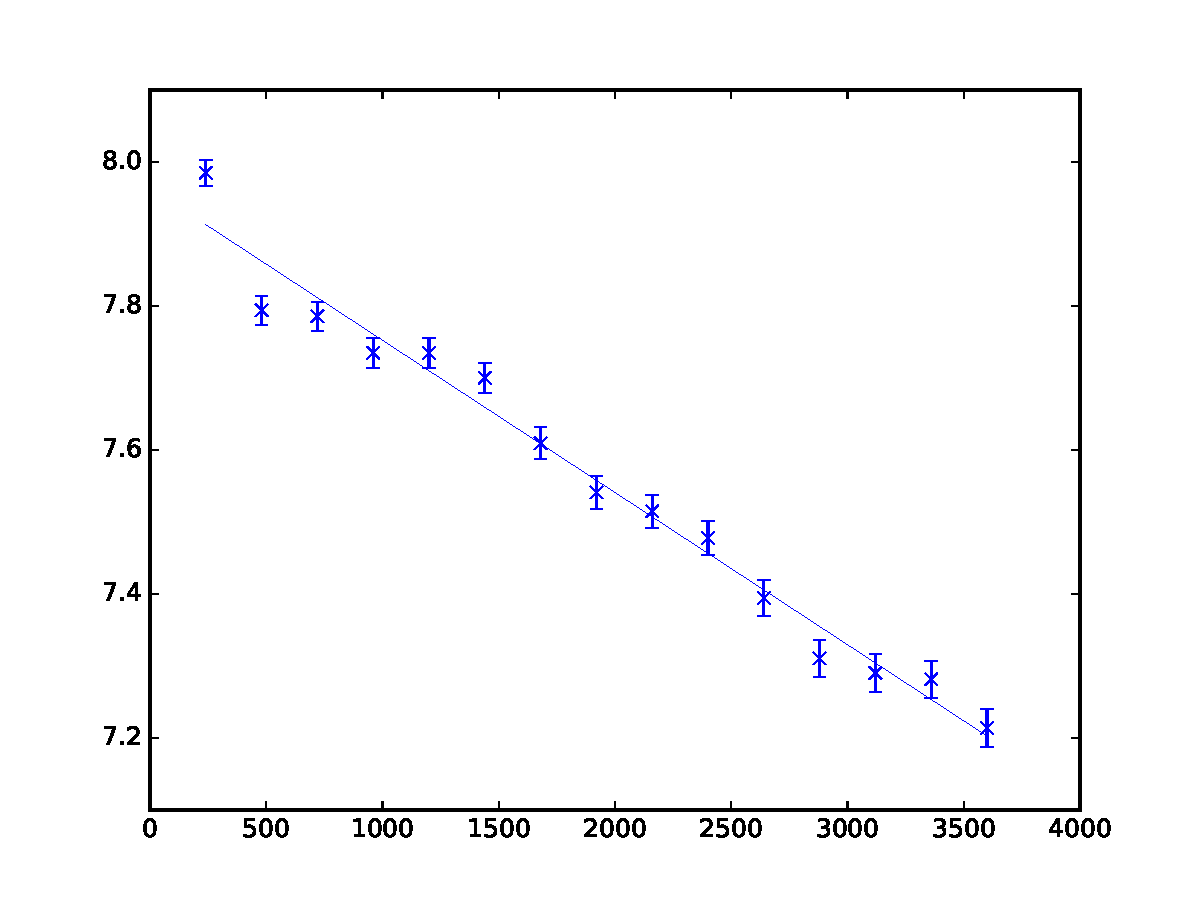
\includegraphics[width = \textwidth]{Indium_log.pdf}
  \caption{logarythmische Darstellung der gemessenen Zerfälle bei Indium}
  \label{fig:Indium}
\end{figure}

Mithilfe einer linearen Regression der Form \eqref{eqn:linRegress} gemäß Formel
?? werden dabei die Zeitkonstante $\lambda$ und $N\ua{0,Indium}$ bestimmt:

\begin{align*}
A &= \lambda\ua{Indium} = (0.0002 \pm 9 \cdot 10^{-6}) \, \frac{1}{\su{s}}\\
B &= N\ua{0,Indium}     = (7.96 \pm 0.02)
\end{align*}

Mit der Formel ?? kann aus der bestimmten Zeitkonstante nun die Halbwertzeit von
Indium bestimmt werden, für die sich der folgende Wert ergibt:

\begin{equation*}
  T\ua{Indium} = (3278 \pm 141) \, \su{s}
\end{equation*}

\subsection{Halbwertzeit von Rhodium}

\begin{figure}
  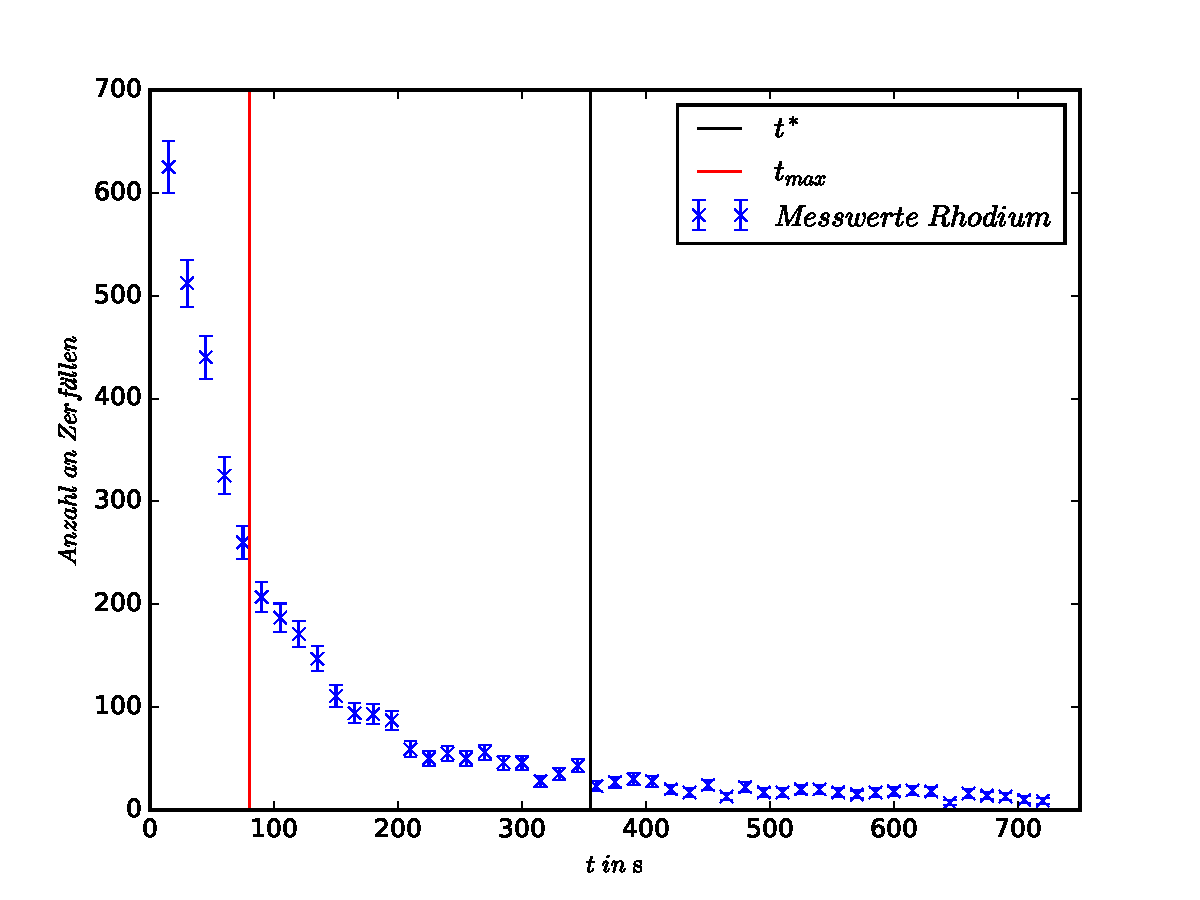
\includegraphics[width = \textwidth]{Rhodium_normal_ohne.pdf}
  \caption{Gemessene Zerfälle bei Rhodium}
  \label{fig:RhodiumOhne}
\end{figure}

Um die Halbwertzeiten der zwei verschiedenen Isotope $Rh^{104}$ sowie $Rh^{104i}$
zu bestimmen, die bei dem Zerfall von $Rh_{45}^{103}$ entstehen, wurden für die
Unterteilung die Messzeiten $t^{*}=355 \, \su{s}$ und $t_i=80 \, \su{s}$ gewählt.





\end{document}
